\documentclass{article}

\usepackage[letterpaper, margin=20mm]{geometry}
\usepackage{hyperref}
\usepackage{graphicx}

\begin{document}

\pagenumbering{arabic}
\begin{center}
{\huge Guide to Android}\\[0.5 cm]
{\large CS 2340, Summer 2018}\\[0.2 cm]
{\large Author: Isaac Weintraub}\\[0.2 cm]
\end{center}
\tableofcontents
\newpage
\section{Introduction}
Unlike in past semesters, Android is \textbf{NOT} required as the platform for your app. However, if your team would like to use Android, feel free to do so. This document outlines the basics of working with Android and creating a simple project.

\section{Getting Started}
You will develop your Android app using the Android Studio IDE. If you have used IntelliJ in CS 1332, you may find Android Studio familiar.\\[0.2cm]
\href{https://developer.android.com/studio/}{\textbf{Download Android Studio here.}}\\[0.2cm]
Once Android Studio is installed, open it. You should see the following screen:
\begin{center}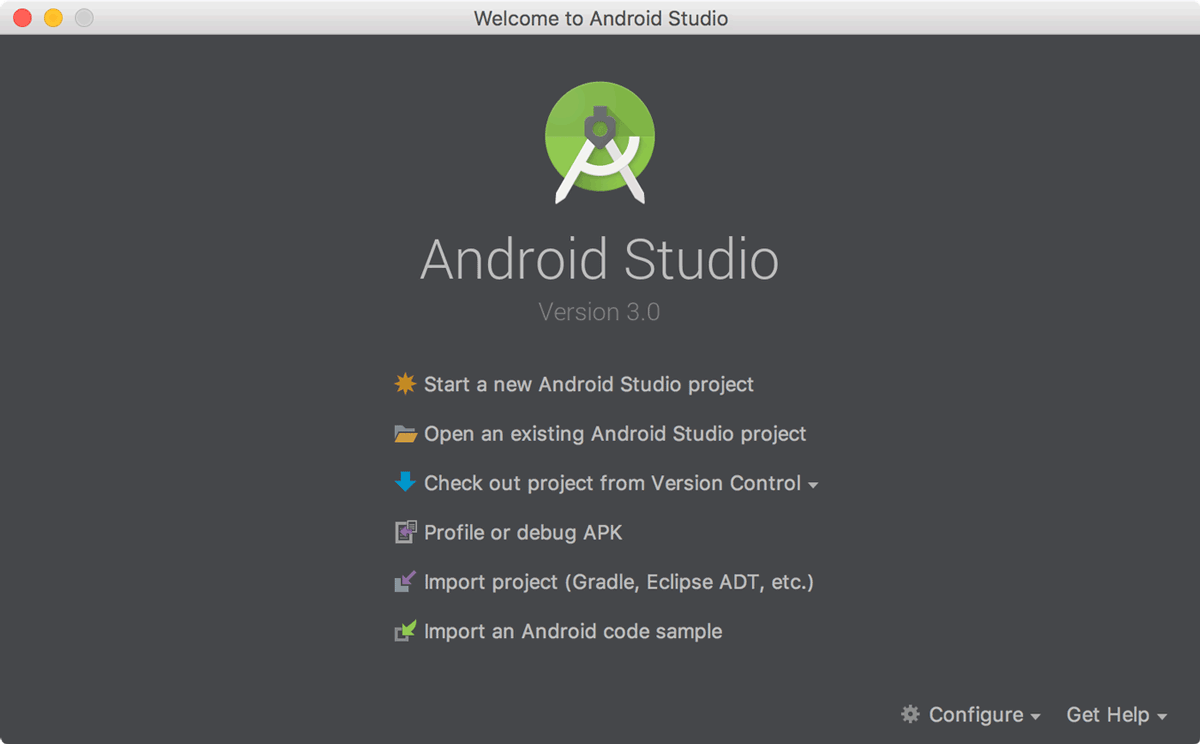
\includegraphics[width=.5\textwidth]{images/studio-open.png}\end{center}
In the window that follows, enter the name for your application, a company domain, and select a location for your project.
\begin{center}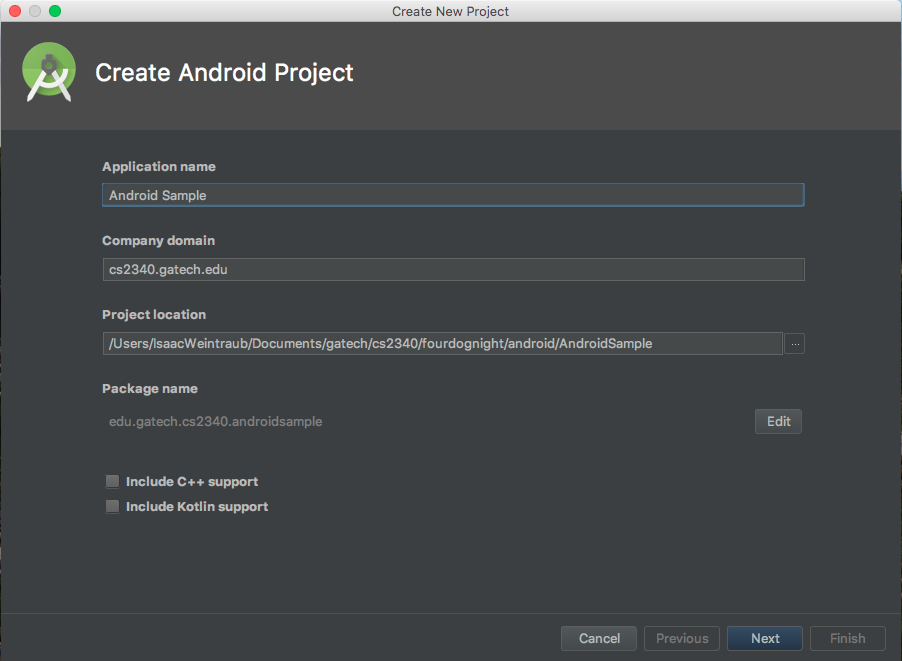
\includegraphics[width=.5\textwidth]{images/create-new.png}\end{center}
Click Next to go to the Target Android Devices screen. Leave Phone and Tablet checked. Choose the API level you want your app to target. Using a newer API level (higher number) will allow your app to use more features, but it will reduce the proportion of devices that your app is compatible with. For the purposes of CS 2340, the API level you target is not important. It is fine to leave the default value, since you can change it later if it becomes necessary to do so. Click Next again to go to the Add an Activity to Mobile screen. Select Empty Activity, and click Next. This will bring you to the Configure Activity screen. You can leave the default values here, and click Finish. The IDE will open after some processing:
\begin{center}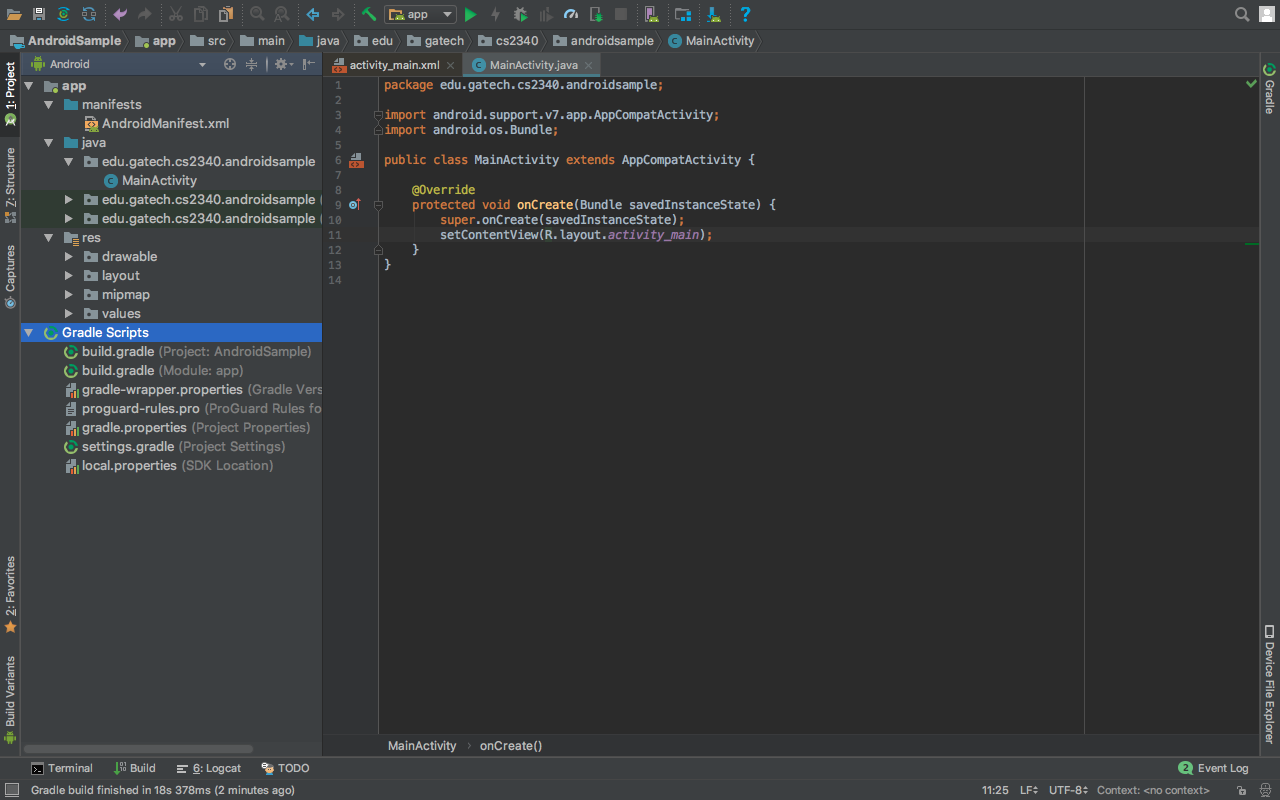
\includegraphics[width=.5\textwidth]{images/ide.png}\end{center}
Select the Project tab at the left of the screen to see your project structure. Here are some important things to observe:
\begin{itemize}
\item \texttt{app > manifests > AndroidManifest.xml} 

This file describes fundamental characteristics of your app, such as the activity that is shown when the app is launched. Manipulation of this file usually happens for you.
\item \texttt{app > java > package name}

This is where your code lives. The package name defaults to being the reverse of the company name you selected followed by the name of your app (e.g. I chose a company name of \texttt{cs2340.gatech.edu} and named my app \texttt{Android Sample}, so the company name that was generated is \texttt{edu.gatech.cs2340.androidsample}).
\item \texttt{MainActivity.java}

In an Android app, different UI screens are organized into activities. These are Java classes that are subclasses of some Android Activity class. The operating system handles the instantiation of your Activities. In this app, the MainActivity that you created when setting up the project is the Activity that is launched when the app is run.
\item \texttt{app > res > layout}

This is where your UI layouts live. These are XML files that define how things are organized on your screen. You will almost always manipulate these using the GUI shown below, and not as raw XML.


\end{itemize}

\section{References}
Some resources you may find useful:
\begin{itemize}
\item Guide to using Android Studio: \url{https://developer.android.com/studio/intro/} 
\item Android development tutorials: \url{https://developer.android.com/guide/} 
\item Android API reference: \url{https://developer.android.com/reference/}
\item Java 7 API specification: \url{https://docs.oracle.com/javase/7/docs/api/} 
\item Java 8 API specification: \url{https://docs.oracle.com/javase/8/docs/api/}
\item Source code for this app: \url{https://github.com/IsaacWeintraub/AndroidSample} 
\end{itemize}
\end{document}